% Options for packages loaded elsewhere
\PassOptionsToPackage{unicode}{hyperref}
\PassOptionsToPackage{hyphens}{url}
%
\documentclass[
  12pt,
]{article}
\usepackage{lmodern}
\usepackage{amssymb,amsmath}
\usepackage{ifxetex,ifluatex}
\ifnum 0\ifxetex 1\fi\ifluatex 1\fi=0 % if pdftex
  \usepackage[T1]{fontenc}
  \usepackage[utf8]{inputenc}
  \usepackage{textcomp} % provide euro and other symbols
\else % if luatex or xetex
  \usepackage{unicode-math}
  \defaultfontfeatures{Scale=MatchLowercase}
  \defaultfontfeatures[\rmfamily]{Ligatures=TeX,Scale=1}
  \setmainfont[]{Times New Roman}
\fi
% Use upquote if available, for straight quotes in verbatim environments
\IfFileExists{upquote.sty}{\usepackage{upquote}}{}
\IfFileExists{microtype.sty}{% use microtype if available
  \usepackage[]{microtype}
  \UseMicrotypeSet[protrusion]{basicmath} % disable protrusion for tt fonts
}{}
\makeatletter
\@ifundefined{KOMAClassName}{% if non-KOMA class
  \IfFileExists{parskip.sty}{%
    \usepackage{parskip}
  }{% else
    \setlength{\parindent}{0pt}
    \setlength{\parskip}{6pt plus 2pt minus 1pt}}
}{% if KOMA class
  \KOMAoptions{parskip=half}}
\makeatother
\usepackage{xcolor}
\IfFileExists{xurl.sty}{\usepackage{xurl}}{} % add URL line breaks if available
\IfFileExists{bookmark.sty}{\usepackage{bookmark}}{\usepackage{hyperref}}
\hypersetup{
  pdftitle={Dams in North Carolina: A Case Study of the Falls Lake Dam},
  pdfauthor={Cheney Gardner and Yingfan Zeng},
  hidelinks,
  pdfcreator={LaTeX via pandoc}}
\urlstyle{same} % disable monospaced font for URLs
\usepackage[margin=2.54cm]{geometry}
\usepackage{graphicx,grffile}
\makeatletter
\def\maxwidth{\ifdim\Gin@nat@width>\linewidth\linewidth\else\Gin@nat@width\fi}
\def\maxheight{\ifdim\Gin@nat@height>\textheight\textheight\else\Gin@nat@height\fi}
\makeatother
% Scale images if necessary, so that they will not overflow the page
% margins by default, and it is still possible to overwrite the defaults
% using explicit options in \includegraphics[width, height, ...]{}
\setkeys{Gin}{width=\maxwidth,height=\maxheight,keepaspectratio}
% Set default figure placement to htbp
\makeatletter
\def\fps@figure{htbp}
\makeatother
\setlength{\emergencystretch}{3em} % prevent overfull lines
\providecommand{\tightlist}{%
  \setlength{\itemsep}{0pt}\setlength{\parskip}{0pt}}
\setcounter{secnumdepth}{5}

\title{Dams in North Carolina: A Case Study of the Falls Lake Dam}
\usepackage{etoolbox}
\makeatletter
\providecommand{\subtitle}[1]{% add subtitle to \maketitle
  \apptocmd{\@title}{\par {\large #1 \par}}{}{}
}
\makeatother
\subtitle{\url{https://github.com/cheneygardner/ENV872-Final-Project.git}}
\author{Cheney Gardner and Yingfan Zeng}
\date{}

\begin{document}
\maketitle

\textbf{Rationale and Research Questions:}\\
According to the Army Corps of Engineers' National Inventory of Dams,
North Carolina has 3191 dams, including the Falls Lake Dam. The Falls
Lake Dam was completed in 1981 to manage the flow of the Neuse River.
Flood control dams remove high flows but can have anthropogenic impacts
on the ecological needs of many aquatic species. For example, if a fish
species has evolved to be triggered to spawn by high flows, a flood
control dam may reduce future reproduction.

Over the past three decades a series of smaller dams downstream on the
Neuse have been removed, and the Neuse River now flows freely from Falls
Lake to the Pamlico Sound for the first time in 100 years. Research has
shown that the removal of these downstream dams has positive ecological
effects. In 2019 shad began migrating all the way to Raleigh for the
\emph{first time} since the 18th century. It is thought that the
migration was potentially triggered by changes in the river flow as
larger flows reduced salinity in estuaries and triggered the fish to
migrate upstream.

\textbf{Question 1:}

*In light of the recent interest in the hydrological effects of dams on
the Neuse River, we wanted to evaluate if there was a change in
discharge before and after the construction of the Falls Lake Dam?
Knowing whether there was a change, and what type or change, is useful
information for ecologists studying the impact of dams on the habitat of
species like shad.

\newpage

\textbf{Dataset Information}\\
\emph{Discharge Data:}\\
To evaluate the change in discharge before and after the construction of
the Falls Lake Dam, we used daily mean discharge data from four USGS
streamflow gages on the Neuse River. The gage data was downloaded from
the USGS National Water Information System.

The date ranges of discharge data available is dependent on the dates in
which the gage has been in use. For example, daily mean discharge data
is available from Gage \#02087183 from 1970 to 2020. Due to seasonality,
we only examined data from full years, ending in 2020. The spatial gage
data was also retrieved from the USGS National Water Information System.

Gage Station Name \textbar{} Gage ID \textbar{} Period Data Available
\_\_\_\_\_\_\_\_\_\_ \textbar{} \_\_\_\_\_\_\_\_\_\_\_ \textbar{}
\_\_\_\_\_\_\_\_\_\_\_ Falls Lake \textbar{} 02087183 \textbar{}
1970-2020 Clayton \textbar{} 02087500 \textbar{} 1927-2020 Goldsboro
\textbar{} 02089000 \textbar{} 1930-2020 Kinston \textbar{} 02089500
\textbar{} 1930-2020

\textbf{Dam Removal Spatial Data}\\
The Falls Lake Dam has recieved increased interest since the removal of
downstream dams, most recently the Milburnie Dam in 2017. To visualize
the downstream dams removed on the Neuse River and others around the
state, we used categorical and spatial data from the American Rivers Dam
Removal Database. The database contains 1,775 entries dating back to
1912, but our sample size was small, as North Carolina contains only 36
removed dams.

We database includes all known dam removals in the U.S. from 1916-2016.
(Note: It is nearly impossible to determine the exact number or dams
removed or when they were constructed because many don't meet the US
Army Corps of Engineers' National Inventory of Dams.) American Rivers
defines a dam as removed if: \emph{a significant portion of the dam must
have been removed for the full height of the dam, such that ecological
function, natural river flow and fish passage can be restored at the
site.}

The dataset contained American Rivers-specific ID, National ID number,
Dam Name, Year Removed, Latitude, Longitude, City and/or County, River,
HUC8, State, Dam Height, Dam Length, Owner, Year Built, Original Use,
Type of Material, Miles Restored and River Miles Reported. For the
purposes of our analysis, we selected only entries from North Carolina
and wrangled only the Dam Name, Year Removed, City and/or County, River,
HUC8 and geometry columns. Two unnamed dams in North Carolina, AR-ID
NC-010 and NC-029, did not have any spatial data, which was critical to
our exploratory analysis, so they had to be removed.

\newpage

\textbf{Exploratory Analysis:}\\
To understand the spatial context of the four gage sites, we mapped the
gage sites, the Falls Lake Dam and the HUC 8 watershed boundaries. (The
HUC 8 hydrologic units were used on both maps because they were
available and relevant for the gage data and dam removal datasets.)
Using Leaflet, we included information on the USGS Station, County and
HUC 8 Subbasin of the gage station, which could be retrieved when the
user interacted with the map. We built functions that allowed us to
customize the coloring and made sure important information, like the
title, did not move when zooming in or out.

Falls Lake Dam and Gage Station Locations used for Discharge Analysis

\begin{figure}
\centering
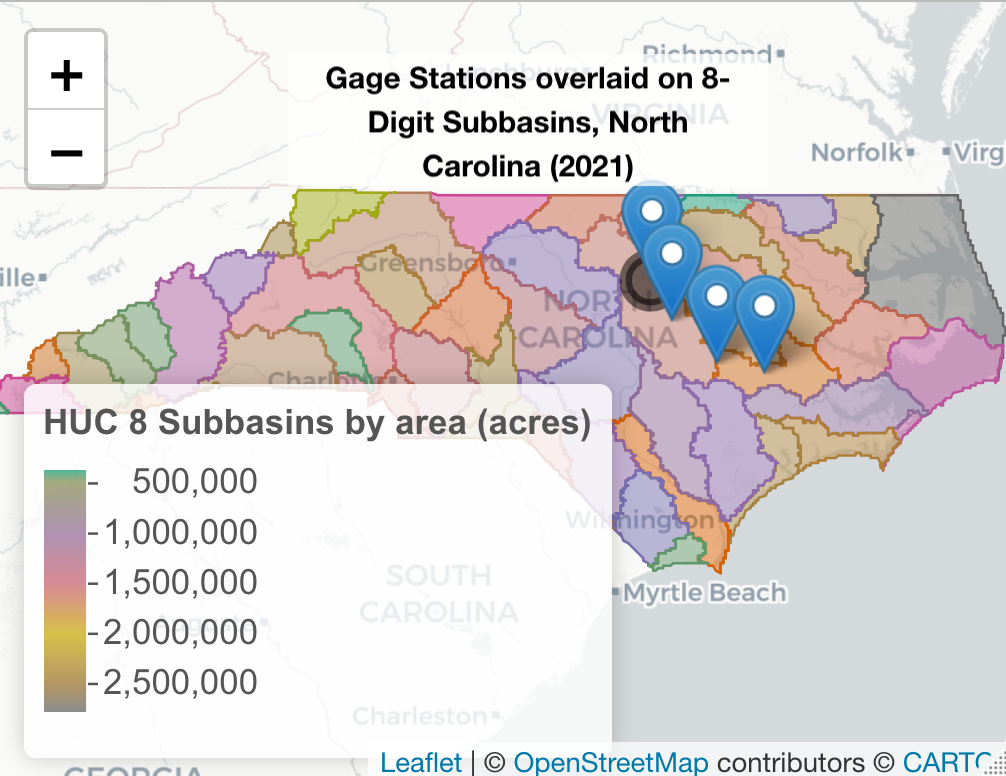
\includegraphics{"./Output/gage.station.png"}
\caption{Gage Stations Analyzed for Falls Lake Dam}
\end{figure}

To visualize the downstream dams removed on the Neuse River and others
around the state, we wrangled American Rivers Dam Removal Database to
only include information from North Carolina. Then we filtered for the
information relevant to our spatial analysis: latitude/longitude, dam
name, removal year and HUC 8 watershed basin.

Dams Removed in North Carolina since 1916, including on Neuse River

\begin{figure}
\centering
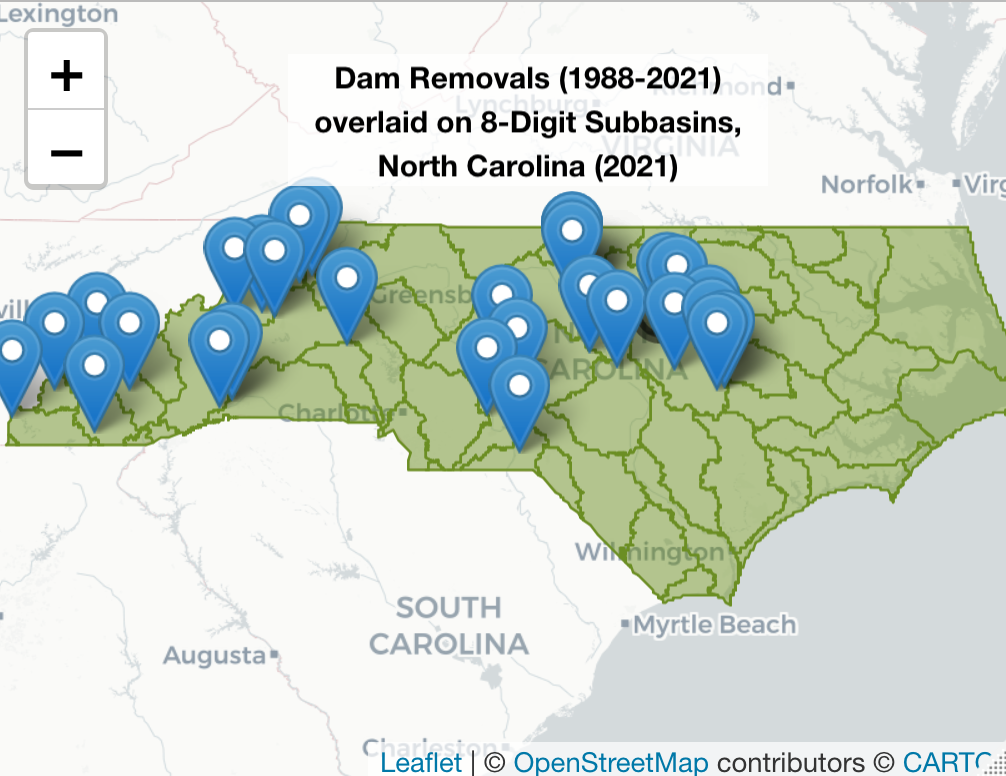
\includegraphics{"./Output/dam.removal.map.png"}
\caption{Dams Removed in North Carolina since 1916}
\end{figure}

When we conducted our analysis of discharge data from the different gage
sites, these maps allowed us to easily determine whether there were
spatial patterns to changes in discharge. The maps also allowed us to
quickly determine which dams on the Neuse had previously been removed,
as well as what other dams in the same HUC watershed.

\newpage

\textbf{Analysis}\\
YZ Time series analysis Generalized linear models T-Test

\newpage

\textbf{Summary and Conclusions}\\
YZ The Falls Lake Dam decreases the downstream discharge, but this
effect diminishes with distance.

\newpage

\#\#References \emph{U.S. Geological Survey, 2016, National Water
Information System data available on the World Wide Web (USGS Water Data
for the Nation), accessed at URL \url{http://waterdata.usgs.gov/nwis/}}

\emph{Rivers, American (2017): American Rivers Dam Removal Database.
figshare. \url{https://doi.org/10.6084/m9.figshare.5234068.v2}}

\end{document}
